\documentclass{article}
\usepackage[margin=1in]{geometry}
\usepackage{../common}
\usepackage{../pagesetup}
\usepackage{tikz}
\usetikzlibrary{bayesnet}
% **** IF YOU WANT TO DEFINE ADDITIONAL MACROS FOR YOURSELF, PUT THEM HERE:

\begin{document}

\lecture{16}{November 1}{Sasha Rush}{ Denis Turcu,Xu Si,Jiayu Yao}{Variational Inference Part 2}

\subsection{Announcements} 
\begin{itemize}
\item T4 out, due 9/13 at 5pm
\item Exams available in office
\item OH - today 2:30-4pm (Wednesdays)
\item  Follow formatting for the abstract of the final project. There were many inconsistencies with the formatting requirements for the initial proposal.
\end{itemize} 

\subsection{Introduction}
Last class, we talked about variational inference. This class, we gonna talk about a very different type of VI. We also will talk about some other types of VI but will not go too much into the details.  \newline

Murphy's book, especially Chapter 22, covers many details on the theory side. The other text, Murphy referred as "The Monster", we put online as a textbook written by Michael Jordan.

\subsection{Bayesian GMM}
We are going to talk more about variational inference. We also put another reference online called VI: A Review for Statisticians. It covers in great detail of Bayesian GMM, so let's write down that model:
\begin{center}
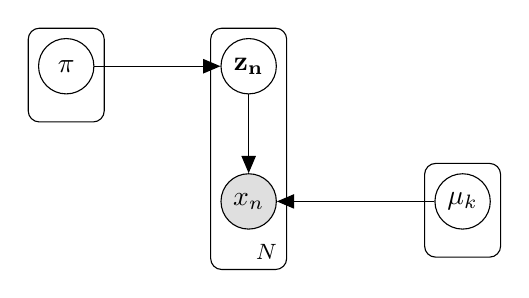
\begin{tikzpicture}

  % Define nodes
  \node[obs]                               (x) {$x_n$};
  \node[latent, above=of x, xshift=0cm]  (z) {$\mathbf{z_n}$};
  \node[latent, left=of z, xshift=-0.6cm] (pi) {$\pi$};
  \node[latent, right=2cm of x]            (mu) {$\mu_k$};

  % Connect the nodes
  \edge {z,mu}{x} ; %
  \edge {pi}{z} ; %

  % Plates
  \plate{}{(mu)}{}
 \plate {}{(pi)}{} 
  \plate {}{(z)(x)}{$N$} ;

\end{tikzpicture}
\end{center}
We assume:
\[ \mu_k \sim \mathcal{N}(0,\sig^2) \;\forall\;k \]
\[ z_n \sim Cat(\f{1}{k}, \dots,\f{1}{k}) \;\forall\; k\]
\[ x_n | z_n, \mu \sim \mathcal{N}(\mu_{z_n},1) \; \forall \; n. \]

Then we write:
\[ p(\{x_n\},\{z_n\},\mu) = p(\mu) \prod_n p(z_n) p(x_n|z_n,\mu). \]
And we get:
\[ p(x) = \int_{z,\mu} p(x,z,\mu) = \int p(\mu) \prod_n \sum_{z_n} p(z_n) p(x_n|z_n,\mu) \rd \mu. \]

{\em Variation setup}. 
Goal:\[ \min_{q\in EASY} KL(q||p) \] 
reverse KL.

We pick $EASY$ as mean field. 
\begin{center}
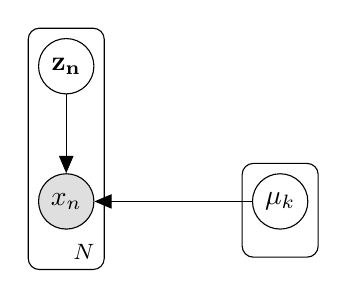
\begin{tikzpicture}

  % Define nodes
  \node[obs]                               (x) {$x_n$};
  \node[latent, above=of x, xshift=0cm]  (z) {$\mathbf{z_n}$};
  \node[latent, right=2cm of x]            (mu) {$\mu_k$};

  % Connect the nodes
  \edge {z,mu} {x} ; %

  % Plates
  \plate{}{(mu)}{}
  \plate {} {(z)(x)} {$N$} ;

\end{tikzpicture}
\end{center}
\begin{center}
p
\end{center}
 
\begin{center}
\begin{tikzpicture}

  % Define nodes
    \node[latent]            (mu) {$\mu_k$};
  \node[latent, left=of x, xshift=-1cm]  (z) {$\mathbf{z_n}$};


  % Plates
  \plate{}{(mu)}{}
  \plate {} {(z)}{} ;
\end{tikzpicture}
\end{center}

\begin{center}
q
\end{center}
Variational parametrization:

\[ q(\mu, z) = \prod_k q_k(\mu_k)\prod_n q_n(z_n). \]

\[ q_n(z_n;\lam_n^{z}) \hspace{2cm} Cat(\lam_n^z). \]
\[ q_k(\mu_k;\lam_k^{\mu}, \lam_k^{\sig^2}) \hspace{2cm} \mathcal{N}(\lam_k^{\mu}, \lam_k^{\sig^2}). \]
\[ \arg \min _{q\in EASY} KL(q||p) = \arg\min_\lam KL \left( \prod_k q_k(\mu_k;\lam_k^{\mu}, \lam_k^{\sig^2}) \prod_n q_n(z_n;\lam_n^{z})  \; || \;  p \right) \] \\ 



"When we do {\em mean field}?"

\[ q_i \sim \exp[ \E_{-q_i} \log(p(z,x)) ]\]

Brief interlude: coordinate ascent $\to$ CAVI (coordinates ascent variational inference). Doing each individual one at a time.
\begin{itemize}
\item Bound we are optimizing is non-convex.
\item This method is monotonically increasing.
\item Sensitive to initialization $\to$ common for random restarts.
\end{itemize}

\bigskip

Example, deriving the math for GMM can be useful to understand how it works and how we will do mean field updates. Start from the above, setup the problem:

\[ \mu_k \sim \mathcal{N}(0,\sig^2) \;\forall\;k \]
\[ z_n \sim Cat(\f{1}{k}, \dots,\f{1}{k}) \;\forall\; k\]
\[ x_n | z_n, \mu \sim \mathcal{N}(\mu_{z_n},1) \; \forall \; n \]

where we also have $\lam_n^z$ for hidden switch variable, and $\lam_k^m, \lam_k^{s^2}$ for the Gaussians.

\begin{align*}
q_n(z_n; \lam_n^z) &\propto exp[\E_{-q_n} \log (p(\mu,z,x))] \\
&\propto exp[\E_{-q_n} \log (p(x_n|z_n, \mu_{z_n}))] \\
&\propto exp[\E_{-q_n} - (x_n - \mu_{z_n})^2 / z] \\
&\propto exp[\E_{-q_n} (x_n\mu_{z_n} - \mu_{z_n}{}^2 / 2)]\\
&\propto exp[x_n \E_{-q_n}(\mu_{z_n}) - \E_{-q_n}(\mu_{z_n}{}^2) / 2]\\
\end{align*}


\begin{center}
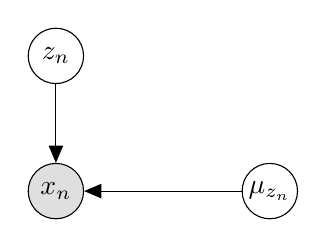
\begin{tikzpicture}

  % Define nodes
  \node[obs]                               (x) {$x_n$};
  \node[latent, above=of x, xshift=0cm]  (z) {$z_n$};
  \node[latent, right=2cm of x]            (mu) {$\mu_{z_n}$};

  % Connect the nodes
  \edge {z,mu} {x} ; %

\end{tikzpicture}
\end{center}

So we identify $ \E_{-q_n}(\mu_{z_n})$ with $\lam_{k=z_n}^m$ and $\E_{-q_n}(\mu_{z_n}{}^2)$ with $\lam_k^{s^2}$, and then we can write:

\begin{align*}
q_k(\mu_k; \lam_{k=z_n}^m, \lam_k^{s^2}) &\propto exp [\E_{-q_n} (\log p(\mu_k) + \sum_n \log p(x_n|z_n,\mu)] \\
&= -\mu_k{}^2 / (2 \sig^2) + \sum_n \E(\log p(x_n|z_n,\mu)) \\
&= -\mu_k{}^2 / (2 \sig^2) + \sum_n \E(z_{nk} (\log p(x_n|\mu_k)) \\
&= -\mu_k{}^2 / (2 \sig^2) + \sum_n \E_{-q_n}(z_{nk}) (\log p(x_n|\mu_k)) \\
&= -\mu_k{}^2 / (2 \sig^2) + \sum_n \lam_{nk}^z  (-(x_n - \mu_{z_n}))^2 / 2 + const. \\
&= (\sum_k \lam_{nk}^z x_n)\mu_k - (\f{\sig^2}{2} + \sum \lam_{nk}^z / 2) \mu_k{}^2 + const. 
\end{align*}

Then:
\[ q_k(\mu_k) = exp[ \tta ^T \phi - A + \dots ], \]
where $\tta_1 = \sum_n \lam_{nk}^z x_n, \; \tta_2 = -(\f{\sig^2}{2} + \sum \lam_{nk}^z / 2$) and $\phi_1 = \mu_k, \; \phi_2 = \mu_k{}^2$, as in GLM.

For normal distribution, we have:
\[ \lam_k^m = \f{\sum_n \lam_{nk}^z x_n}{1/\sig^2 + \sum_n \lam_{nk}^z}, \trm{ and } \lam_k^{s^2} = \f{1}{1/\sig^2 + \sum_n \lam_{nk}^z}. \]

\subsection{Exponential Family}

\[ p(z_j|z_{-j},x) = h(z_j) exp(\tta^T\phi(z_j) - A(\tta)), \]
where $\tta$ are function of $z_{-j}, x$. One nice case is {\em UGM}:

\begin{center}
\begin{tikzpicture}

  % Define nodes
  \node[latent]       (mid) {$z_j$};
  \node[latent, above=of mid, yshift=0.5cm]  (up) {};
  \node[latent, below=of mid, yshift=-0.5cm]  (below) {};
  \node[latent, left=of mid, xshift=-0.5cm]  (left) {};
  \node[latent, right=of mid, xshift=0.5cm]  (right) {};

  % Connect the nodes
  \edge[-] {up} {mid} ;
  \edge[-] {right} {mid} ;
  \edge[-] {below} {mid} ;
  \edge[-] {left} {mid} ;

\end{tikzpicture}
\end{center}
\begin{center}
blanket
\end{center}


\[ q(z) = \prod_j q(z_j)\]
\begin{align*}
q(z) &\propto exp[\E_{-q_j} \log p(z_j|z_{-j},x)] \\
&\propto exp[ \log(h) + \E(\tta)_{z_j}^T - \E (A(\tta))] \\
&\propto h(z_j) exp[\E(\tta)^T z_j]
\end{align*}

where $\E(\tta)^T$ are the natural parameters of the variational approximation \newline
\[\lambda_j = \E[\theta(z_{-j},x)]\]

\subsection{Latent Dirichlet Allocation}
\begin{itemize}
\item Widely used generative latent variable model
\item generative model set up
\begin{center}
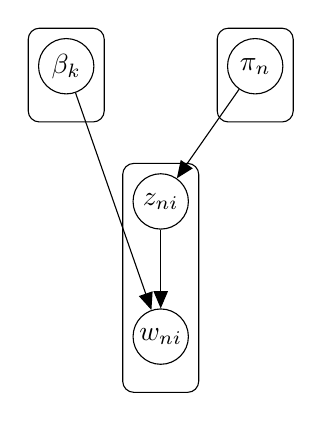
\begin{tikzpicture}

  % Define nodes
  \node[latent]                               (w) {$w_{ni}$};
  \node[latent, above=of w, xshift=0cm]  (z) {$z_{ni}$};
  \node[latent, above=of z, xshift=-1.2cm] (beta) {$\beta_k$};
  \node[latent, above=of z, xshift=1.2cm]            (pi) {$\pi_n$};

  % Connect the nodes
  \edge {z} {w} ; %
  \edge {beta} {w} ; %
  \edge {pi} {z} ; %

  % Plates
  \plate{}{(beta)}{}
 \plate {} {(pi)} {} 
  \plate {} {(z)(w)} {} ;

\end{tikzpicture}
\end{center}
where $\be_k \sim Dir(\eta)$, $\pi_n \sim Dir(\alpha)$, $z_{ni} \sim Cat(\pi_n)$, $w_{ni} \sim Cat(\be_{z_{ni}})$
\item Topic molding story: 
\begin{itemize}
\item $n$ - documents
\item $i$ - words
\item $\pi_n$ - document topic distribution
\item $\be_k$ - topic-word distribution
\item $z_{ni}$ - topic selected for word $i$ of document $n$ 
\item $w_{ni}$ - word selected for $ni$. 
\item $\lam_{ni}^z$ - probability for the topic of word $i$ in document $n$
\end{itemize}
 


\end{itemize}

\subsection{Demo}

\smallskip
We did an example iPython notebook (\href{https://github.com/harvard-ml-courses/cs281-demos/blob/master/TopicModeling.ipynb}{\texttt{TopicModeling.ipynb}}) in class.



\end{document}
